%! Author = leona
%! Date = 09/02/24
% !TeX root = ../thesis-main.tex

\chapter{Background}
\label{chap:background}

\section{Internet of Things and Pervasive Computing}

\subsection{The Definition of IoT}
The \ac{iot} is a broad and ever-evolving field that has its roots in the concept proposed in 1999 by Kevin Ashton where he refers to it as ``uniquely identifiable
interoperable connected objects with \ac{rfid} ''. As the years passed, the scope of IoT evolved with the rapid increase in the rate of computational power and
chip size and now it denotes an intricate, wide system of interconnected devices that become 'smart' or 'intelligent' through added sensors and computational capabilities.
Within the IoT, ``physical and virtual ‘things’ have identities and attributes and are capable of using intelligent interfaces and being integrated as an information network” (IERC 2013; Kirtsis 2011; Li et al.
2012a, b)''.

\subsection{From mobile computing to Pervasive Computing}

\section{Collective Adaptive Systems}

\section{Field Calculus}

\section{Aggregate Programming}

\section{The ScaFi Framework}

\section{The Rust Programming Language}
The Rust Programming Language\cite{002} is a multi-paradigm, general-purpose programming language designed originally for systems-level development. It strives to achieve both execution
speed and memory safety and efficiency while providing zero-cost abstractions and high-level features that are unusual for low-level programming languages such as C or C++.
In this section, we will go through Rust's main features and asses whether this language is suitable to develop an \acs{ac} implementation that can run on thin devices or not.

\subsection{Rust's Basic Features}
\subsubsection{Variables and mutability}
Like the majority of today's programming languages, Rust supports storing values inside variables for referencing them in various sections of the program. \\
The developer can store a value inside a variable through a \textit{let} statement:

\begin{lstlisting}[language=Rust]
    let x = 5;
\end{lstlisting}

There is an interesting thing to notice in this piece of code: Rust is a statically typed language, but the type of the variable can be omitted thanks to the type inference mechanism. This means that the compiler can figure out the type of the variable by looking at the value assigned to it. In this case, the type of \textit{x} is \textit{i32}, which is a 32-bit signed integer. \\

Another important feature of Rust variables is that they are immutable by default. This means that once a value is assigned to a variable, it cannot be changed.
For example, the following code will not compile:

\begin{lstlisting}[language=Rust]
    let x = 5;
    x = 6; // error: cannot assign twice to immutable variable `x`
\end{lstlisting}

Instead, the developer can opt out of the mutability by using the \textit{mut} keyword:

\begin{lstlisting}[language=Rust]
    let mut x = 5;
    x = 6; // this code compiles
\end{lstlisting}

\subsubsection{Data Types}
The Rust Language supports a wide range of data types that can be both found in low-level programs and in high-level designs. These data types can be divided into two main categories: scalar types and compound types.
For scalar types, the following are supported:
\begin{itemize}
    \item \textbf{Integers}: both signed and unsigned integers of different sizes. In particular, rust supports 8, 16, 32, 64, and 128-bit signed and unsigned integers;
    \item \textbf{Floating-point numbers}: both 32 and 64-bit floating-point numbers;
    \item \textbf{Booleans}: a boolean type that can be either \textit{true} or \textit{false};
    \item \textbf{Characters}: the language's most primitive alphabetic type, represented by a single Unicode scalar value.
\end{itemize}

For compound types, the following are supported:
\begin{itemize}
    \item \textbf{Tuples}: the simplest form of product type in Rust, represented by a collection of values of possibly different types;
    \item \textbf{Arrays}: a collection of values of the same type. Unlike other languages, Rust arrays have a fixed length.
\end{itemize}

In addition to these compound types, Rust offers several other collections; for example:

\begin{itemize}
    \item \textbf{Vectors}: a collection of values of the same type. Unlike the arrays, Rust vectors have a dynamic length;
    \item \textbf{Strings}: a growable UTF-8 encoded string type;
    \item \textbf{Hash Maps}: a collection of key-value pairs, implemented as a hash table.
\end{itemize}


\subsection{The Ownership System}
Rust's Ownership System is its most unique feature and is a core part of how the language achieves memory safety without the need for a garbage collector.
The term \textit{ownership} refers to a set of rules that govern how a program's memory is managed and it is enforced by the compiler, meaning that if
a program violates them, it won't compile. This means that none of these features will cause runtime overhead for the program.

\subsubsection{Ownership Rules}
The Rust's ownership rules are the following:

\begin{enumerate}
    \item Each value in Rust has an owner.
    \item There can only be one owner at a time.
    \item When the owner goes out of scope, the value will be dropped.
\end{enumerate}

This means that a variable's validity (and presence in memory) is tied to the scope of the variable's owner: when the owner's scope is over, the compiler will automatically
call the drop function on every owned variable, freeing the memory associated with it and making it so that the variable is no longer valid.

\subsubsection{Moving and Copying}
The ownership system has implications on what happens when a variable of a certain type is copied. For example in the following code:

\begin{lstlisting}[language=Rust]
    let x = 5;
    let y = x;
\end{lstlisting}

The value of \textit{x} is copied into \textit{y}. This means that there are now two variables on the stack both with the value of 5. This is possible because x is an integer-type variable,
and integers have a fixed and known size at compile time, so they can be pushed cheaply onto the stack.

However, if we analyze the following code:

\begin{lstlisting}[language=Rust]
    let s1 = String::from("hello");
    let s2 = s1;
\end{lstlisting}

Since s1 is a String type, which does not have a known size at compile time, s1 will consist of a pointer in the stack, pointing to a heap-allocated memory that contains the actual string data, as shown in the figure \ref{fig:string-memory-rep}.

\begin{figure}[h]
    \centering
    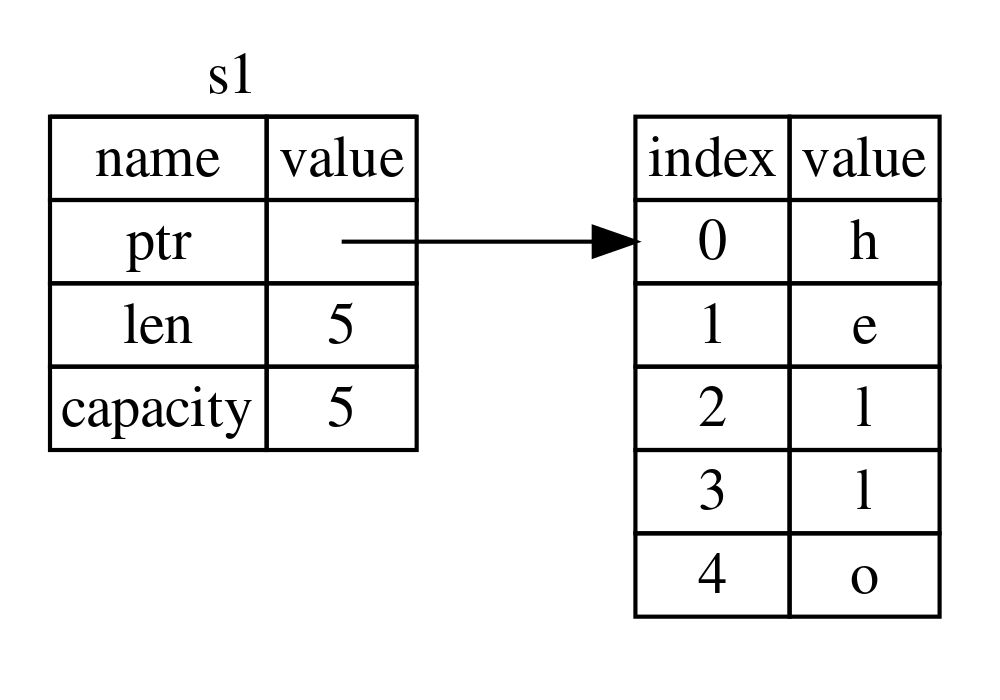
\includegraphics[width=0.5\textwidth]{figures/string-memory-rep.png}
    \caption{Representation of the memory layout of a string in Rust}
    \label{fig:string-memory-rep}
\end{figure}

When s1 gets copied into s2, only the pointer in the stack is copied, so that the memory layout of the program will look like the one in figure \ref{fig:string-memory-rep2}.

\begin{figure}[h]
    \centering
    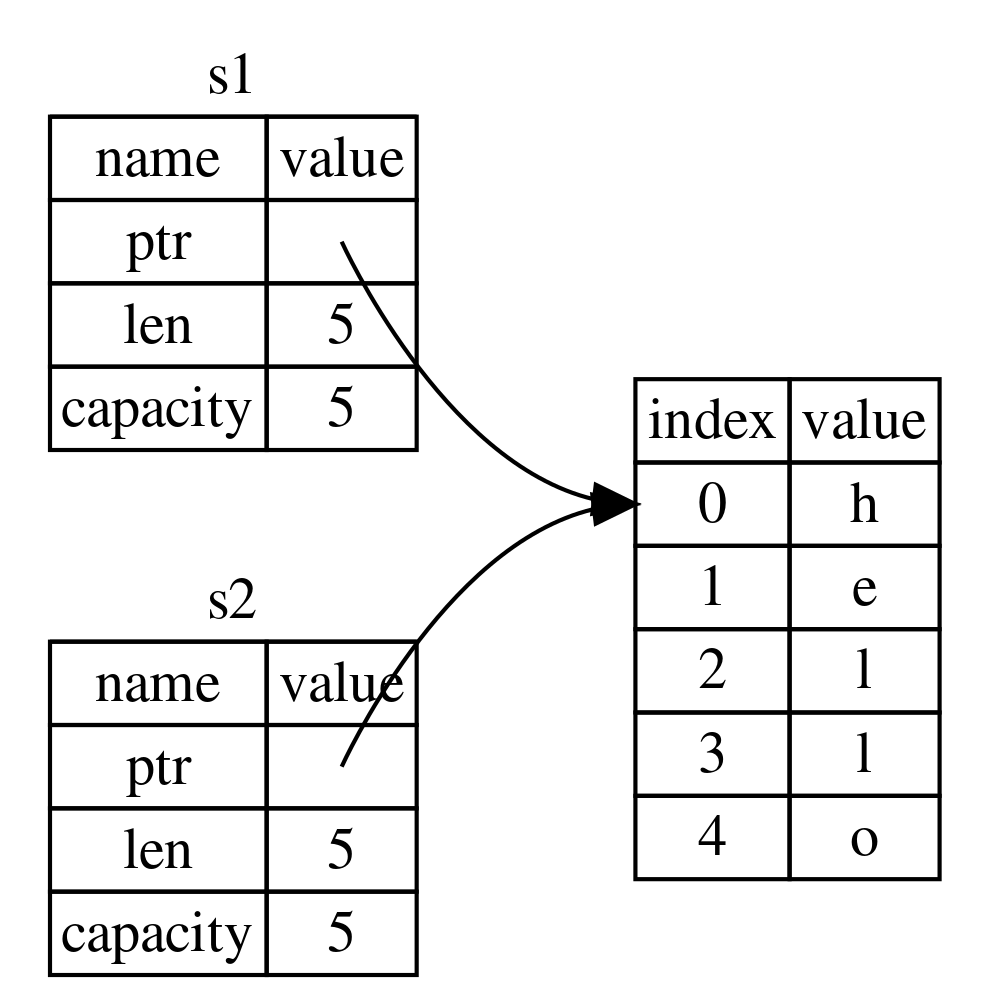
\includegraphics[width=0.5\textwidth]{figures/string-memory-rep-2.png}
    \caption{Representation of the memory layout of a string in Rust after the copy}
    \label{fig:string-memory-rep2}
\end{figure}

According to the ownership rules, when s1 and s2 go out of scope, one may think that the memory will be freed twice, causing a double-free error. However, in reality, after the copy, the compiler
will not consider s1 to be valid anymore, so when s1 goes out of scope, the memory will be freed only once, as shown in figure \ref{fig:string-memory-rep3}.

\begin{figure}[h]
    \centering
    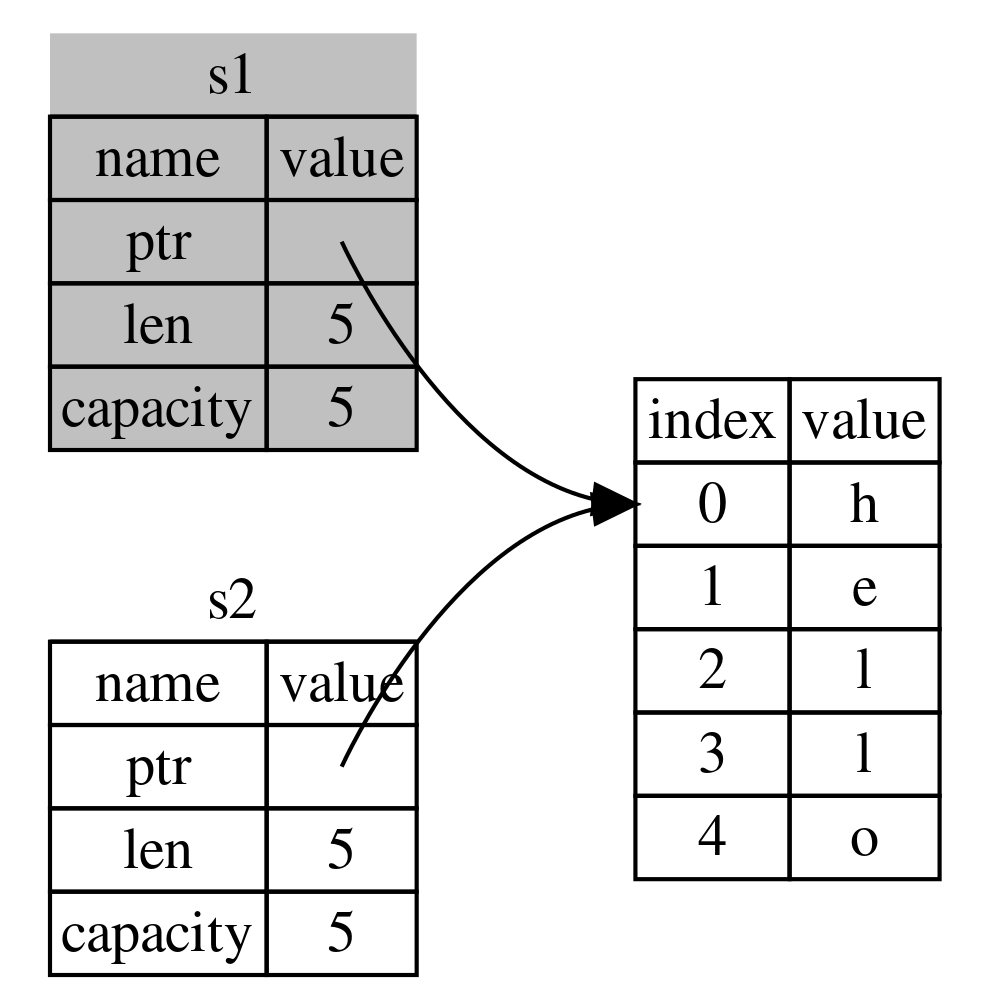
\includegraphics[width=0.5\textwidth]{figures/string-memory-rep-3.png}
    \caption{Representation of the memory layout of a string in Rust after the copy and the end of the scope of s1}
    \label{fig:string-memory-rep3}
\end{figure}

In this case, it is said that the variable s1 has been \textit{moved} into s2. This means that s1 is no longer valid and cannot be used anymore.
This happens because, by default, Rust doesn't create deep copies of variables of types that don't have a known size at compile time. After all, creating a deep copy of such
a variable would cause the allocation of a new memory block on the heap, an expensive operation both in terms of execution time and memory usage. If the developer
needs to create deep copies of variables stored in the heap, they can explicitly use the \textit{clone} method, which will create a new memory block on the heap and copy the data into it.

\subsubsection{Ownership and Functions}
Similarly to what happens during the variable assignment, passing a variable to a function will cause it, depending on its type, to be moved or copied, as shown in the listing \ref{lst:func_own_1}.

\lstinputlisting[language=Rust, label={lst:func_own_1}]{listings/function_ownership_ex1.rs}

Returning values from functions will also cause ownership to be transferred, as shown in the listing \ref{lst:func_own_2}.

\lstinputlisting[language=Rust, label={lst:func_own_2}]{listings/function_ownership_ex2.rs}

\subsubsection{References and Borrowing}
Instead of taking ownership of a variable and then returning it to the caller, it is possible to pass a reference to the variable to the function, so that the function can use the variable without taking ownership of it.
For a function to take a reference to a variable, it is sufficient to prefix the type definition of the variable with an ampersand (\&).
By default, references are immutable, meaning that the function cannot modify the value of the variable. If the function needs to modify the value of the variable, it is possible to take a mutable reference to it by using the \&mut keyword.

\subsection{Functional Features of Rust}
In this subsection, we will discuss some of the \ac{fp}-adjacent features of Rust.

\subsubsection{Product Types}
In FP, product types are types that combine n values of possibly different types. In Rust, it is possible to define Product types by using the \textit{struct} keyword. In particular, one can define a product type in two ways as shown in the listing \ref{lst:product_types}.

\lstinputlisting[language=Rust, label={lst:product_types}]{listings/product_types.rs}

It is also possible to add functionality to the ADTs created by using the \textit{impl} keyword, as shown in the listing \ref{lst:product_types_impl}.

\lstinputlisting[language=Rust, label={lst:product_types_impl}]{listings/product_types_impl.rs}

\subsubsection{Sum Types and Pattern Matching}
In FP, a sum type represents a choice between some types. In Rust, we can define Sum types by using the \textit{enum} keyword. It is also possible to perform pattern matching over a sum type, as it is shown in the listing \ref{lst:sum_types}.

\lstinputlisting[language=Rust, label={lst:sum_types}]{listings/sum_types.rs}

\subsubsection{Polymorphism}
Rust supports polymorphism through traits. Rust's traits are similar to Haskell's typeclasses and they allow us to define a particular functionality that a particular type has.
For example, we can implement Haskell's Show typeclass in Rust as shown in the listing \ref{lst:polymorphism}.

\lstinputlisting[language=Rust, label={lst:polymorphism}]{listings/polymorphism.rs}

\subsubsection{Lambdas and Closures}
In FP, lambda functions or anonymous functions, are functions that are not bound to a name. Moreover, closures are lambda functions that can "capture" the environment in which they are defined.
In Rust, both lambdas and closures are supported, though they are both called closures. Like in other languages, Rust closures can be assigned to variables and passed to functions.
When defining a closure in Rust, it is important to reason about the ownership of the variables that are captured by it. The listing \ref{lst:closures} shows some examples of closures in Rust.

\lstinputlisting[language=Rust, label={lst:closures}]{listings/closures.rs}

\subsubsection{Iterators}
The Iterator pattern allows to traverse collection of elements in a particular manner, performing some task on each element in turn. The iterator is responsible for the trasversal logic
so that the developer doesn't need to reimplement it each time. In Rust, the Iterator pattern is implemented through the \textit{Iterator} trait, which is implemented by the standard library's collections:

\begin{lstlisting}[language=Rust]
    trait Iterator {
        type Item;
        fn next(&mut self) -> Option<Self::Item>;
        //Other default methods omitted
    }
\end{lstlisting}

The developer can also implement the Iterator trait for his custom types, enabling many functionalities that are divided into the following categories:

\begin{itemize}
    \item \textbf{Consumer Adaptors}: these are methods that take ownership of the iterator because they traverse it using its next method, thus consuming it. Examples of consumer adaptors are reducing methods like \textit{sum};
    \item \textbf{Iterator Adaptors}: these are methods that don't take ownership of the iterator, since they take an iterator and return another, modified one. An example of an iterator adaptor is the \textit{map} method, which applies a function to each element of the iterator;
\end{itemize}

\subsection{Why Rust}
As shown in the previous sections, Rust is a general-purpose programming language designed with a focus on safety, speed and efficiency. These design principles, coupled with high-level features
more adjacent to functional programming than to low-level programming, make Rust a good candidate for developing \ac{ac} implementations that can run on thin devices.


\section{Towards a Rust-based AC Implementation: the RustFields Project}